\chapter{Alternatives} \label{alternatives}
Nix isn't the only declarative solution to system management, but is a
rare example of \textit{purely functional package manager} Another
such package manager is Guix. Guix also comes with it is related
distribution GuixOS. Guix has many features in common with Nix, but
the configuration language is GNU Scheme instead of Nix language. Guix
isn't, at least yet as mature as NixOS, but claims to correct most of
NixOS's faults from its historical payload. In this chapter, however
two alternative architectures are presented as a reference. Note that
many more imaginable architectures could be depicted, but only two of
possible architectures are displayed. \cite{dolstra2010nixos}
\cite{courtes2013functional}

\section{Alternative updatable architecture 1.}
One alternative for declarative system would be a device fleet with
Gentoo Linux. As Portage allows rsyncing binaries and sources as a
out-of-the-box solution, this would allow synchronous update system
between the central server and the device fleet. Portage handles
dependency issues well, so it could be used as a host for other
solutions. A sample figure of the partial architecture is shown in
figure \ref{gentooarchitecture} \cite{thiruvathukal2004gentoo}
\begin{figure}[H]
\centering
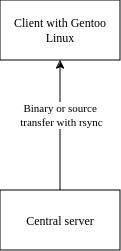
\includegraphics[scale=0.8]{latex/kuvat/gentooarchitecture.drawio.png}
\caption{A minimal architecture, where synchronisation is achieved
  with rsync.}
\label{gentooarchitecture}
\end{figure}

\section{Alternative updatable architecture 2.}
Container tools, such as Docker and Podman are useful for predictable
software deployment, but they as they lack pure functionality, they
can suffer from same kind of problems as imperative package managers
usually do. One solution regarding updatability would be a stable
Linux host system, perhaps a Gentoo Linux, and hosting the needed
services via Docker/Podman as shown in figure
\ref{dockerarchitecture}. Updates to the kernel would be trivial with
Portage, and the whole user-space would reside in a container or
multiple containers. This would perhaps add a layer of security
through isolation.
\begin{figure}[H]
\centering
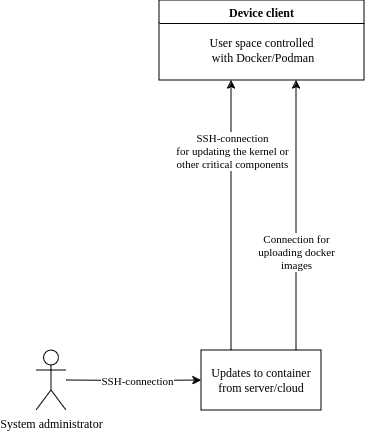
\includegraphics[scale=0.7]{latex/kuvat/dockerarchitecture.drawio.png}
\caption{Sample server-client architecture graph of client containing
  a Docker image}
\label{dockerarchitecture}
\end{figure}

\section{Security perspectives}
These two architectures could have the same type of security layering
as the project in \ref{architecture}. If the user-space would mainly
reside in a Docker container, some isolation could be achieved as
mentioned in the previous section. This would restrict unprivileged
users, and would reduce the risks, when a device is partially
compromised. In architecture 1, this could be achieved via appropriate
user privileges or the use of chroot-jails.
